\section{Diseño de la interfaz}

En esta sección se describe como se ha diseñado la interfaz de usuario de la aplicación. En primer lugar, se realizó un {\it mockup} \cite{mockup} de un par de páginas de la aplicación para comprobar que la apariencia era la deseada por parte de los expertos jurídicos.
\\

La estructura y guía de colores están basados en los utilizados en la página web de lex.gal. En esta, se utilizan como colores principales el azul, blanco, gris y negro. En cuanto a la estructura, se coloca a la izquierda de todas las páginas una barra lateral donde se encontrará el nombre de la aplicación, así como distintas opciones a realizar dentro de la página. Por su parte, el contenido en todas ellas abarcará todo el resto de la página.

\begin{figure}[H]
\centerline{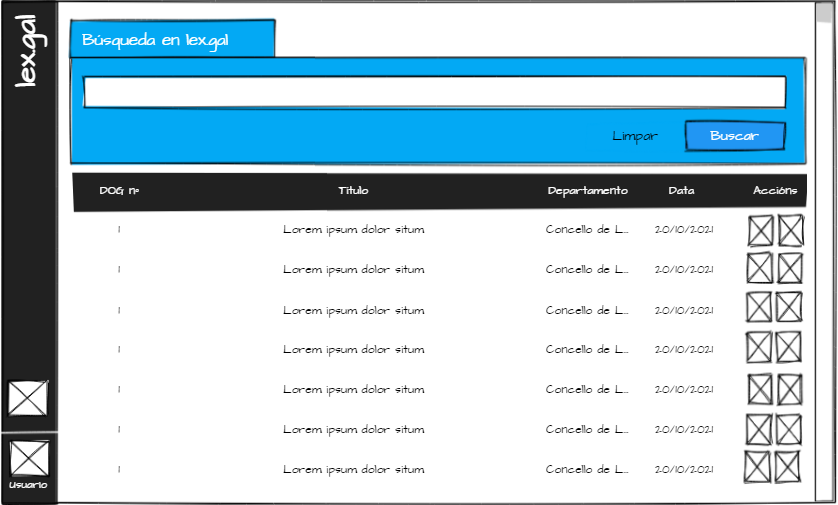
\includegraphics[width=15cm]{figuras/diseño/MockupBusquedas.PNG}}
\caption{Diseño inicial de la página de búsqueda de leyes en lex.gal.}
\label{enlaceMockupPrincipalDiseno}
\end{figure}

Se puede observar en la \hyperref[enlaceMockupPrincipalDiseno]{Figura 3.7} un primer diseño de la página de búsquedas. En esta destacan un buscador en la parte superior de la aplicación, y, debajo de este buscador, se muestran las leyes encontradas en una tabla.

\begin{figure}[H]
\centerline{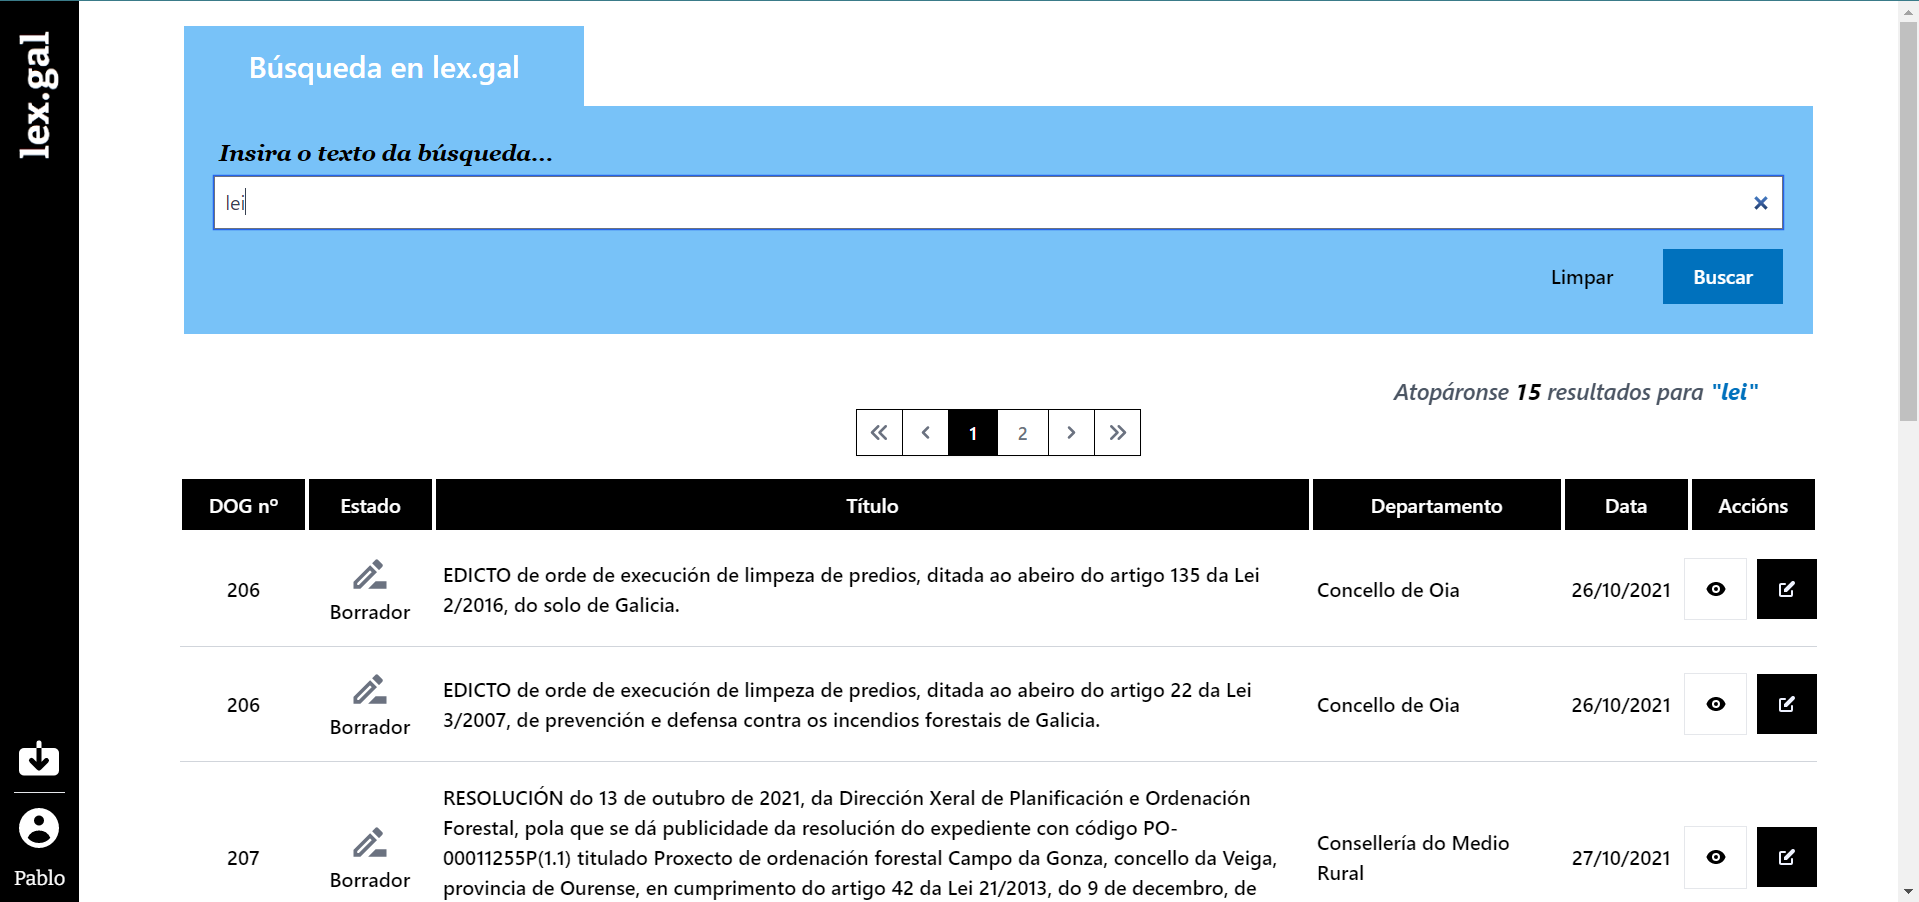
\includegraphics[width=15cm]{figuras/diseño/PPrincipalDiseno.PNG}}
\caption{Diseño final de la página de búsqueda de leyes en lex.gal.}
\label{enlacePPrincipalDiseno}
\end{figure}

El resultado final de esta página varió ligeramente, añadiendo un mayor número de elementos, como se puede observar en la figura \hyperref[enlacePPrincipalDiseno]{Figura 3.8}. En ella, se muestra, al igual que en el primer diseño, el buscador y la tabla de leyes. No obstante, se ha añadido que se muestre el número de resultados encontrados para el texto buscado, se permite navegar entre páginas y se ha añadido la columna de estado de la ley.

\begin{figure}[H]
\centerline{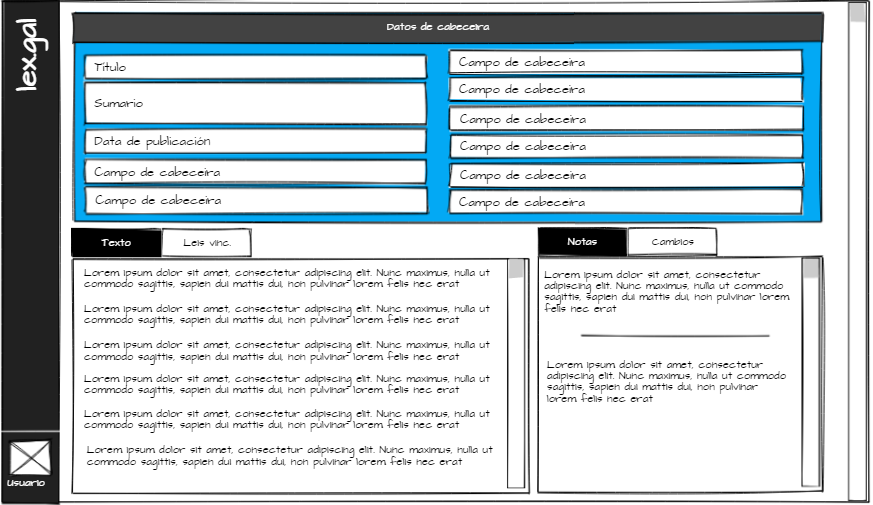
\includegraphics[width=15cm]{figuras/diseño/MockupEdicion.PNG}}
\caption{Diseño inicial de la página de edición de una ley de lex.gal.}
\label{enlaceMockupEdicionDiseno}
\end{figure}

Otra página de la que se realizó un primer diseño fue la página de edición. El {\it mockup} realizado se puede observar en la \hyperref[enlaceMockupEdicionDiseno]{Figura 3.9}. En este caso, se podían localizar los datos de cabecera en la parte superior de la página, el texto de la ley principal a la izquierda, donde se podía cambiar a la pestaña de leyes vinculadas, y, a la derecha, navegación entre notas y cambios.

\begin{figure}[H]
\centerline{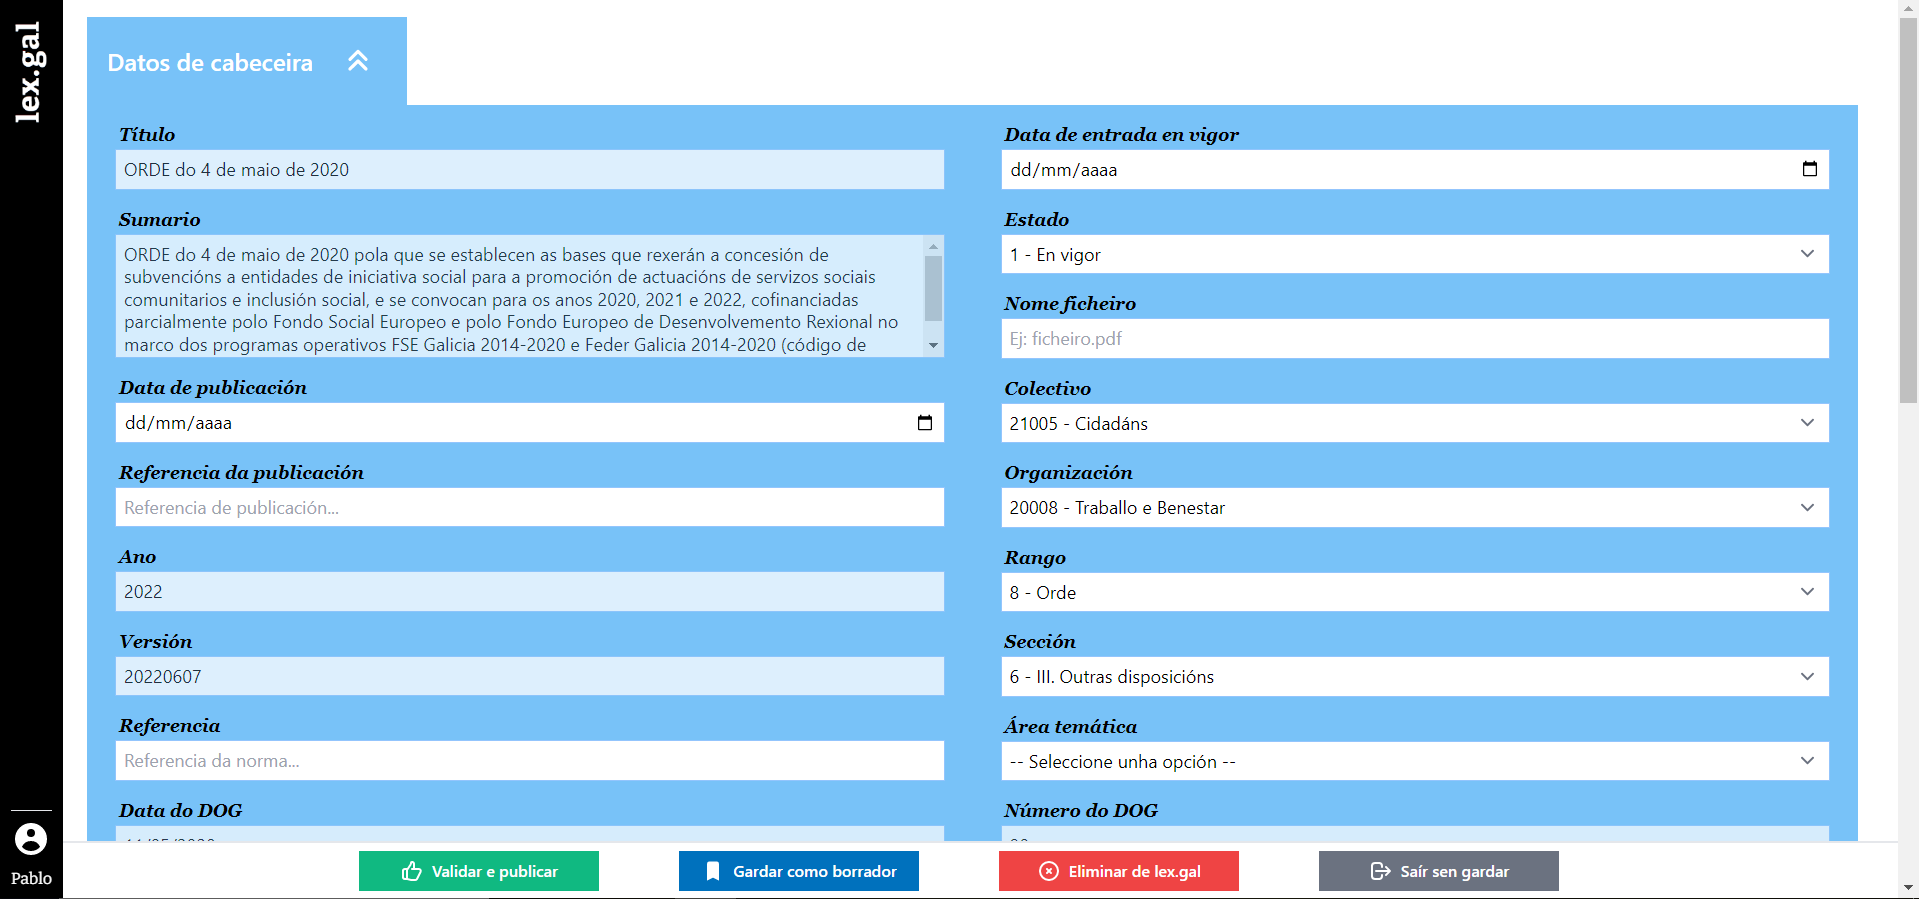
\includegraphics[width=15cm]{figuras/manualUsuario/EditarCabecera.PNG}}
\caption{Diseño final de la página de edición de una ley de lex.gal - I.}
\label{enlaceCabeceraDiseno}
\end{figure}

\begin{figure}[H]
\centerline{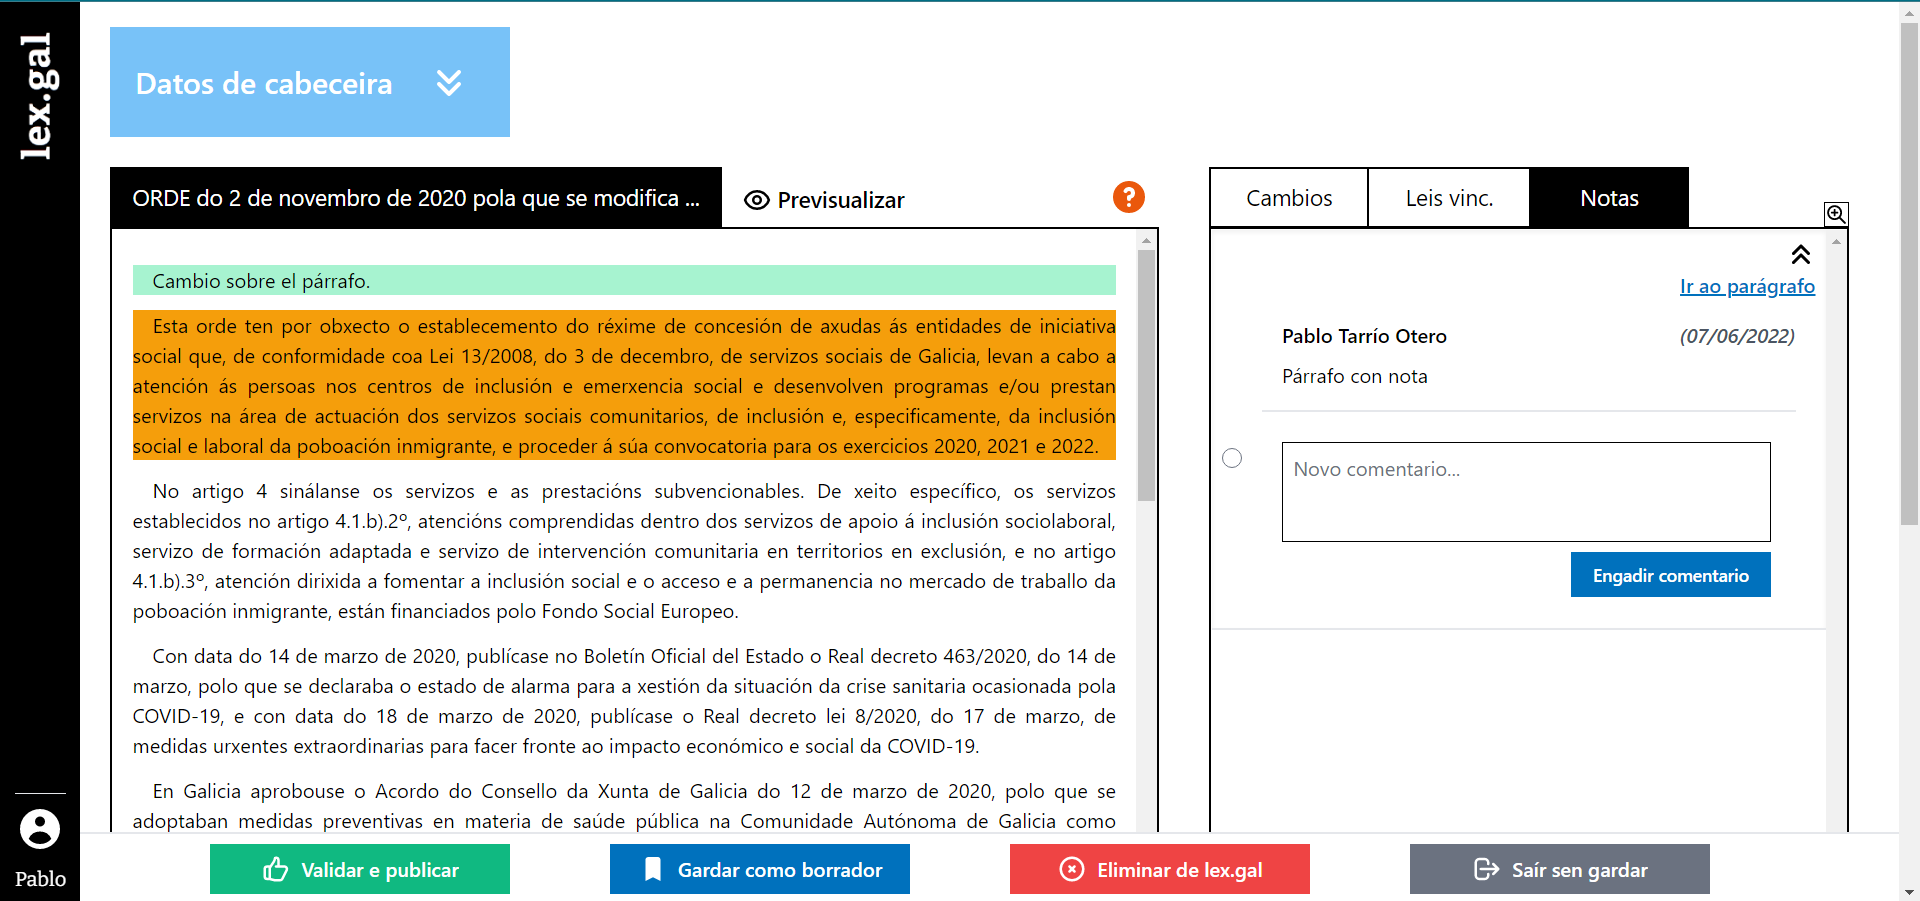
\includegraphics[width=15cm]{figuras/manualUsuario/PestanaNotas.PNG}}
\caption{Diseño final de la página de edición de una ley de lex.gal - II.}
\label{enlaceEdicionLexGalDiseno}
\end{figure}

En la \hyperref[enlaceCabeceraDiseno]{Figura 3.10} y en la \hyperref[enlaceEdicionLexGalDiseno]{Figura 3.11} se puede ver el resultado final de la página de edición. Se observa a simple vista que esta cambió bastante con respecto a su diseño inicial.
\\

En primer lugar, el número de datos de cabecera era muy amplio, con lo que se consideró hacer un desplegable según se quisieran ver o no. El siguiente cambio aparente fue mostrar un fragmento del sumario encima del texto, para poder saber qué ley se está editando. Sobre el texto de esta ley, se pueden añadir cambios (párrafos con fondo de color verde), y añadir anotaciones sobre párrafos (párrafos con color naranja de fondo).
\\

En cuanto a la parte de la derecha, se han movido a esta parte las leyes vinculadas. Esto se debe a que en todo momento el experto en textos jurídicos desea ver el texto sobre el que trabaja, y en el caso del {\it mockup}, si quería ver las leyes vinculadas, este dejaba de ver el texto de la ley. 
\\

Por su parte, las notas y cambios ahora aparecen comprimidos para que el usuario trate de reconocerlos a simple vista, y en caso de querer más información, desplegarlos. También se permite acceder al párrafo donde se realizan, lo cual antes no se contemplaba. Esto se realiza guardando el párrafo sobre el que se realiza la nota/cambio, y la página realiza un scroll automático al párrafo correspondiente. Además, ahora sobre las notas también se permiten añadir comentarios.
\\

Por último, se han añadido en la parte inferior de la página cuatro botones que se mantendrán siempre en dicha posición. Estos botones permitirán realizar diferentes operaciones sobre las leyes que se editan, ya sea validarlas, guardar como borrador, o eliminar.

\begin{figure}[H]
\centerline{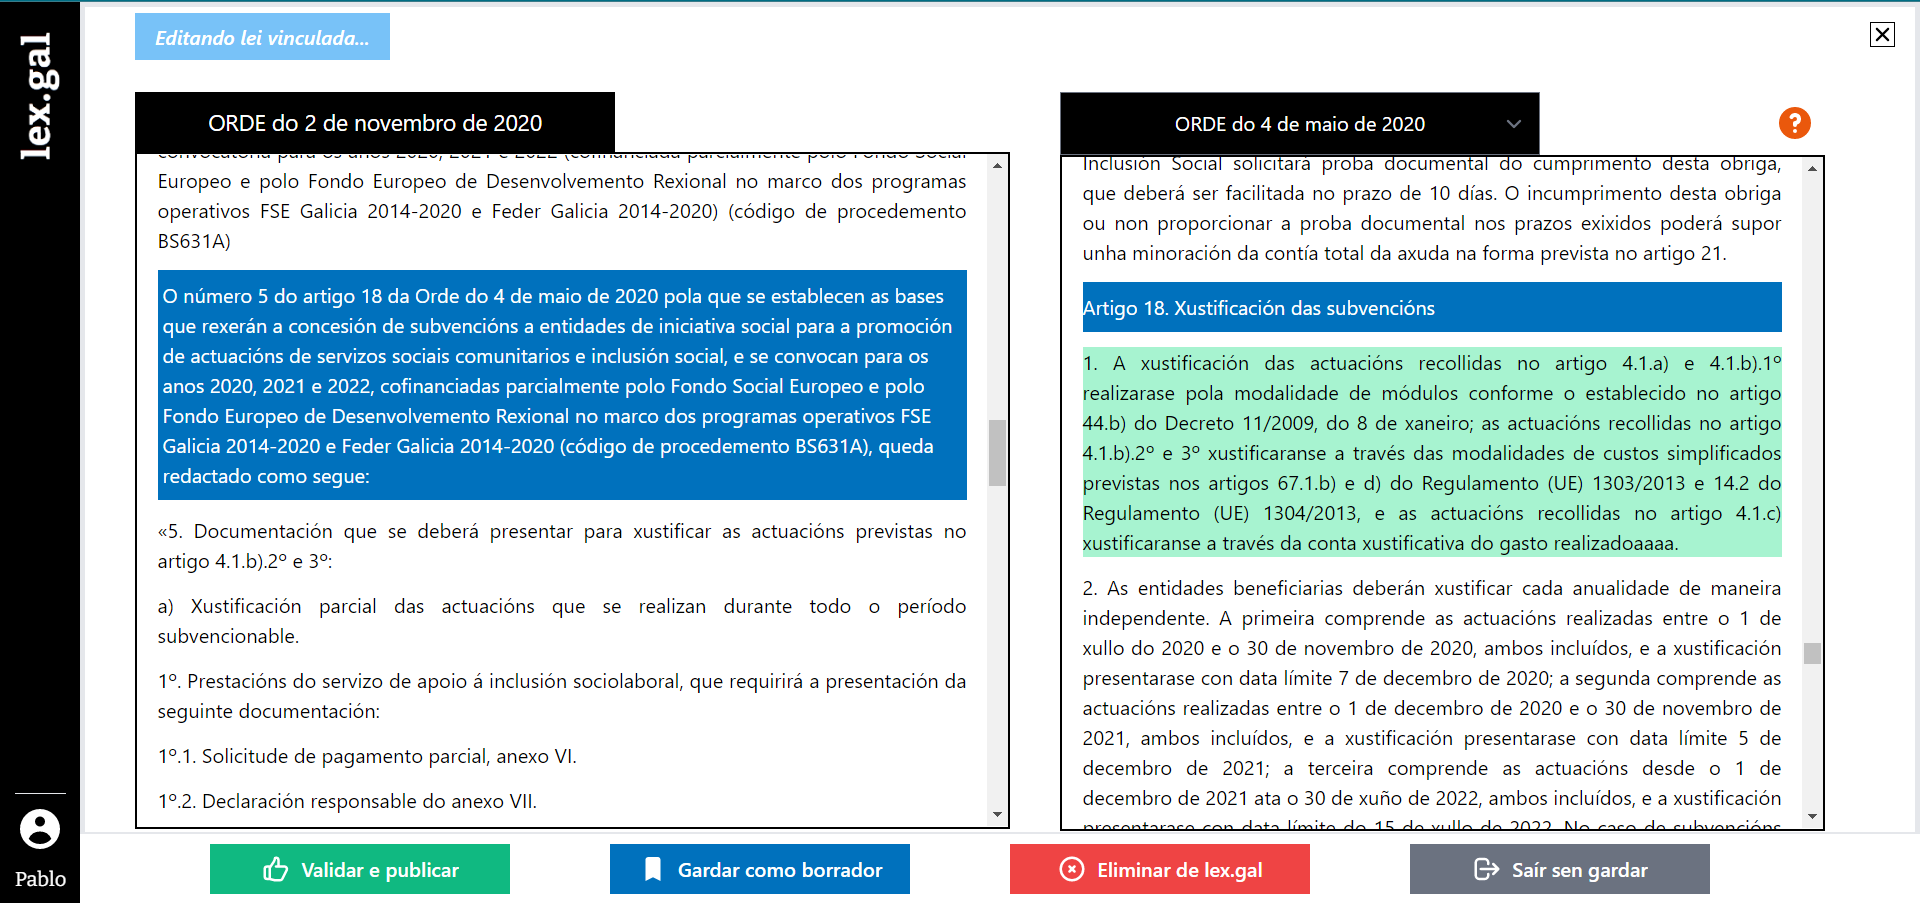
\includegraphics[width=15cm]{figuras/manualUsuario/PestanaLeyVinculada.PNG}}
\caption{Diseño de la pestaña de edición de leyes vinculadas.}
\label{enlacePLeyVinculadaDiseno}
\end{figure}

Por último, también cabe destacar el diseño de la pestaña de edición de una ley vinculada, si bien de esta no se hizo un diseño en su versión inicial al ser una funcionalidad que no se planteó al inicio del proyecto. Este diseño se puede ver en la \hyperref[enlacePLeyVinculadaDiseno]{Figura 3.12}.
\\

En ella, se puede observar la ley principal (izquierda), donde se localizan cambios que se realizan sobre la ley vinculada (derecha). Estos cambios son localizados mediante expresiones regulares que detectan frases sobre el texto de la ley principal (por ejemplo, ``queda redactado como segue''). Si se pincha en el párrafo con fondo azul, se redirigirá al usuario a la parte de la ley vinculada donde se realiza el cambio, también detectado mediante el uso de expresiones regulares (por ejemplo, detección de ``Artigo 18''). Si se realiza un cambio sobre un párrafo, este quedará marcado con un fondo de color verde.